\documentclass{VUMIFPSkursinis}
\usepackage{algorithmicx}
\usepackage{algorithm}
\usepackage{algpseudocode}
\usepackage{amsfonts}
\usepackage{amsmath}
\usepackage{bm}
\usepackage{caption}
\usepackage{paralist}
\usepackage{color}
\usepackage{float}
\usepackage{graphicx}
\usepackage{listings}
\usepackage{subfig}
\usepackage{wrapfig}
\usepackage{enumitem}% http://ctan.org/pkg/enumitem

% Titulinio aprašas
\university{Vilniaus universitetas}
\faculty{Matematikos ir informatikos fakultetas}
\department{Programų sistemų katedra}
\papertype{Kursinis darbas}
\title{Gestų kalbos atpažinimas naudojant įprastą web kamerą}
\titleineng{Sign language recognition using web camera}
\status{3 kurso I grupės studentas}
\author{Pranciškus Ambrazas}
\supervisor{asist. Linas Petkevičius}
\date{Vilnius, \the\year}

% Nustatymai
% \setmainfont{Times New Roman}   % Pakeisti teksto šriftą į Palemonas (turi būti įdiegtas sistemoje)
\bibliography{bibliografija}

\begin{document}
\maketitle

\tableofcontents

\sectionnonum{Įvadas}
Daugiau nei 360 milijonų žmonių pasaulyje kenčia dėl klausos ir kalbos įvairių problemų, o daugiau 32 milijonai jų yra vaikai ir šis skaičius vis auga \cite{http://www.who.int/mediacentre/factsheets/fs300/en/}. Gestų kalba yra pagrindinis šių žmonių bendravimo įrankis. Tačiau reiktų pastebėti ir tai, jog dalis jų moka skaityti iš lūpų. Norint žmogui be šių ydų bendrauti su gestakalbiu (\textit{gestų kalba kalbantis žmogus}) reikia vertėjo, kuris išverstų gestų kalbą į įprastinę ir atvirkščiai.

Kiekviena pasaulyje esanti kalba turi ir savo gestų kalbą.Tai reiškia, skiriasi tiek gestų kalbos gramatika, tiek netgi patys gestai. Pasaulyje randama net dialektų pagal regionus, ne tik pagal šalis. Pavyzdžiui, amerikiečių anglų kalba šnekančių žmonių pasaulyje yra apie 500 tūkstančių \cite{remiantis United States Census Bureau’s data from the 2009-2013 American Community Survey}. Todėl netgi bendraujant dviem žmonėms, mokantiems gestų kalbą neretai iškyla vertimo problema, tad tenka ieškoti gestų vertimų. Paiešką galima atlikti atsižvelgiant į delno padėtį, rankos judesį (ar net abiejų rankų), rankos padėtį ir kiek rankų atlieka gestą. Tuomet pagal gesto išvaizdos paveiksliukus ar kartais net vaizdo įrašus, gestakalbiai gali išsiversti gestus. Tam yra skirtos tiek internetinės svetainės - žodynai, tiek įvairūs rašytiniai žodynai.

Šio tyrimo tikslas - padėti ne tik gestakalbiams tarpusavyje, bet ir žmonėms, nesuprantantiems gestų kalbos bendrauti su gestakalbiais tam pasitelkiant technologijas, taip suteikiant šiems žmonėms pilnavertį gyvenimą bendraujant su kitais. Šiuo tyrimu siekiama apžvelgti ir įvertinti ar naudojantis įprasta kompiuterine kamera įmanoma paversti gestų kalbą rašytiniu tekstu ar net garsine kalba ir lygiai taip pat versti rašytinę ar garsinę kalbą į gestų kalbą. Taip pat siekiama, kad vėliau būtų sukurtas visiems gestakalbiams prieinamas produktas ar programinė įranga, kurią kiekvienas įsidiegęs į savo įrenginį - kompiuterį, mobilųjį telefoną ar planšetinį kompiuterį galėtų naudotis šiuo vertėju. Taip pat tai galėtų tapti ir mokomąja gestų kalbos priemone. 

Šiuo metu yra gaminamas vienas iš tokių produktų, tačiau tai yra atskiras įrenginys, turintis įmontuotą kamerą, kuri be vaizdo taip pat fiksuoja ir atstumą iki tam tikrų objektų (šiuo atveju rankos), tačiau produkto kūrėjai sako, jog jų įrenginys galės versti gestų kalbą į anglų ir kitas kalbas ir lygiai taip pat versti įprastą kalbą į rašytinę kalbą. Plačiau: \textit{http://www.motionsavvy.com/}





%Įvade apibūdinamas darbo tikslas, temos aktualumas ir siekiami rezultatai.
%Darbo įvadas neturi būti dėstymo santrauka. Įvado apimtis 1–2 puslapiai.
\section{Apsimokančios sistemos ir gestų kalba}
\subsection{Apsimokančios sistemos}
\textbf{Apsimokančios sistemos} (\textit{angl. machine learning}) - tai mokslas apie tai, kaip kompiuterius užprogramuoti taip, jog jie patys darytų sprendimus be žmogaus įsikišimo neužprogramuojant kiekvienos galimos situacijos. Kitais žodžiais tariant leisti kompiuteriui pačiam nuspręsti kaip elgtis esant tam tikroms aplinkybėms. Dar kitaip tariant tai yra pradžia norint sukurti dirbtinį intelektą. 

Savaime apsimokančių sistemų ir jų algoritmų sukūrimo dėka gatvėmis pradėjo važinėti pačios save vairuojančios (\textit{angl. self-driving cars} arba dar kitaip vadinamos autonominės transporto priemonės, įvairūs paieškos varikliai tokie kaip „Google“ ar „Yahoo“ taikydami šiuos alogirtmus naudojams rodo kiekvienam asmeniškai sugeneruotą turinį. Taip pat reikėtų paminėti ir kalbos atpažinimo sistemas tokias kaip „Siri“ ar „Google Assistant“, kurios iš joms duotų komandų atlieka tam tikrus veiksmus.

\subsection{Gestų kalba}
\subsubsection{Gestų kalbos skirstymas}
Gestų kalba susideda iš dviejų dalių - statinių ir dinaminių ženklų. Statiniais ženklais atvaizduojama didžioji abėcėlių raidžių dalis. O dinaminiais - žodžiai ir kai kurios gestų abėcėlių raidės. \textit{Pavyzdžiui}, amerikiečių gestų kalbos abėcėlėje J ir Z raidės atvaizduojamos dinaminiais judesiais (\textit{žr. 1 pav.}), o lietuvių - Ą, D, Į, K ir kt. (\textit{žr. 2 pav.})

\begin{figure}[H]
\centering
\begin{minipage}{.5\textwidth}
    \centering
    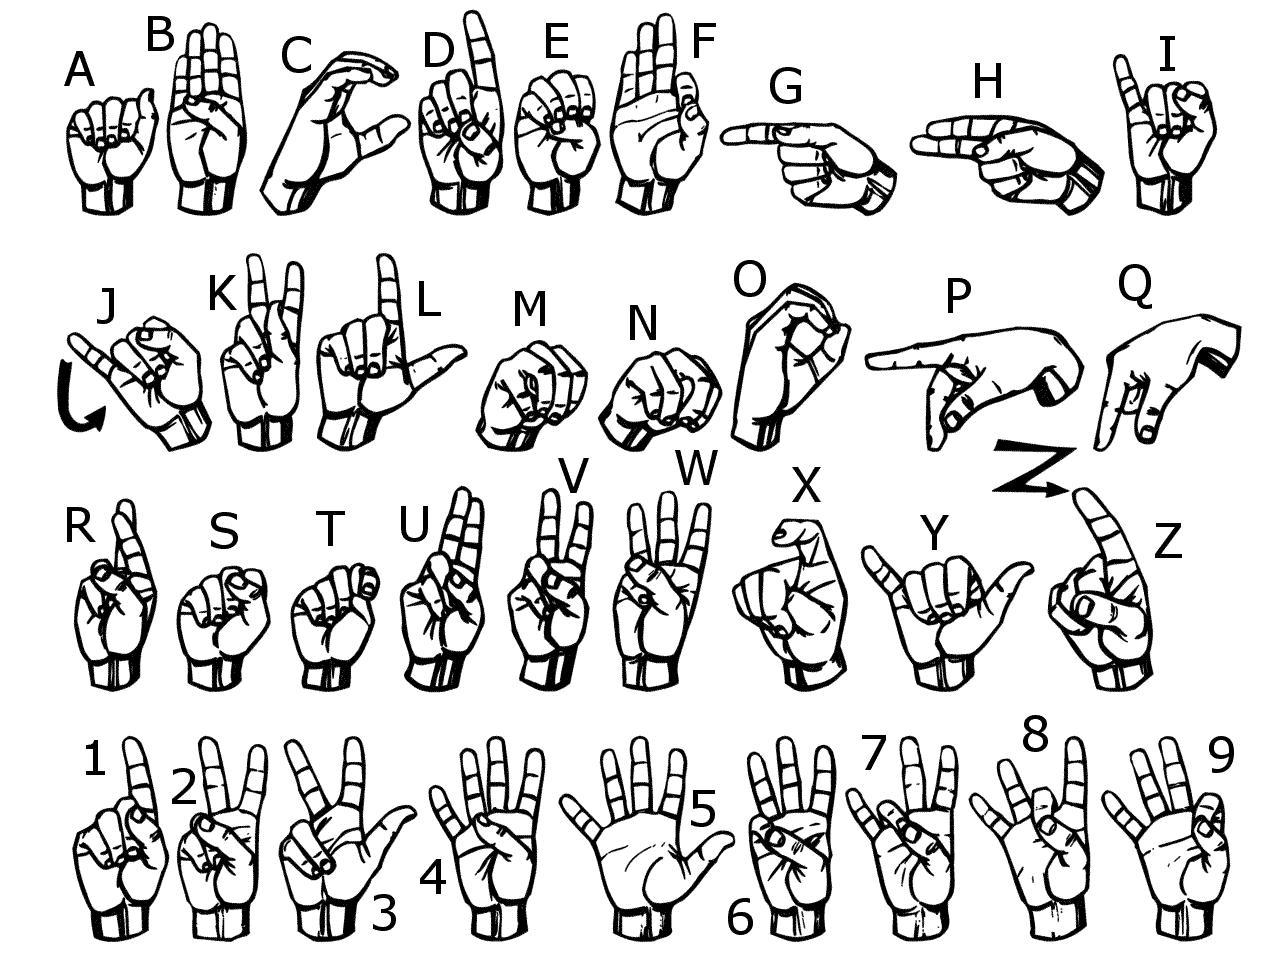
\includegraphics[width=.8\linewidth]{img/asl_alphabet}
    \caption{Amerikiečių gestų kalbos abėcėlė}
    \label{img:asl_alphabet}
    %http://lifeprint.com/asl101/topics/wallpaper1.htm
\end{minipage}%
\begin{minipage}{.5\textwidth}
    \centering
    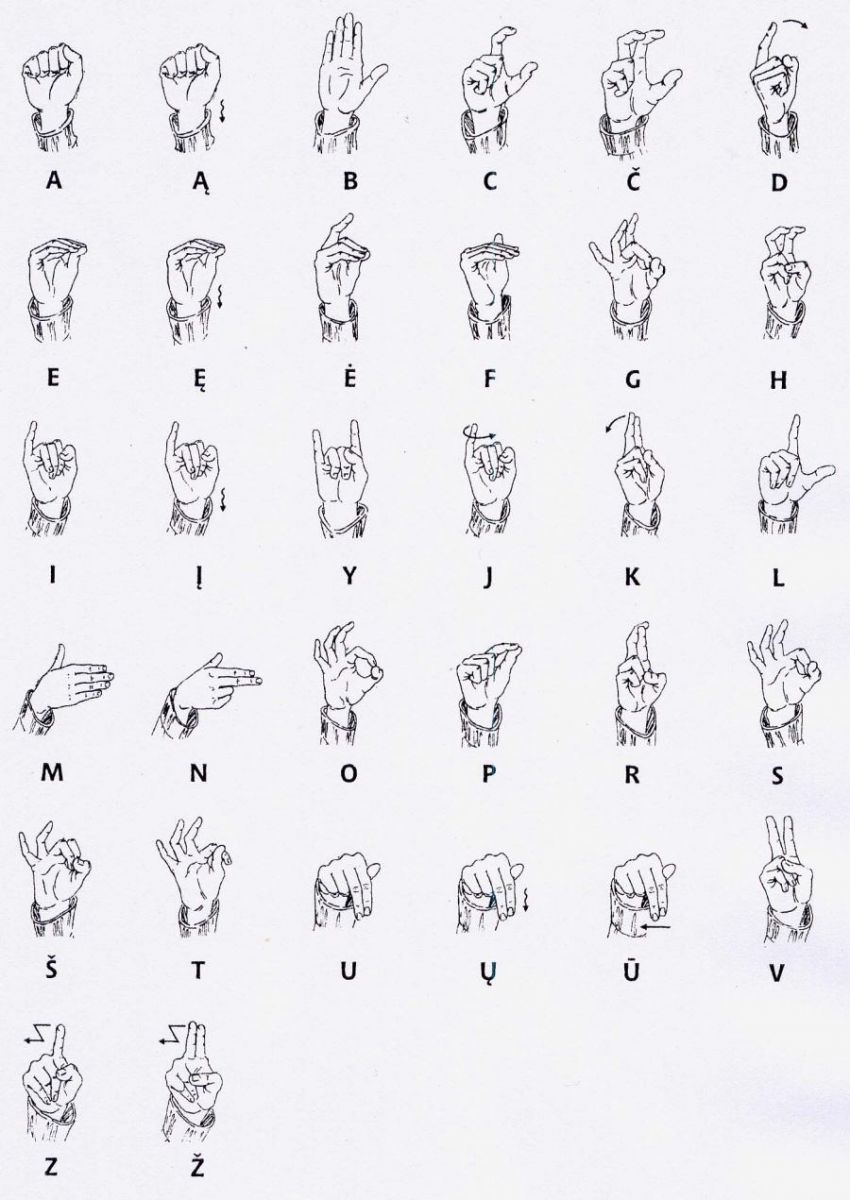
\includegraphics[width=.5\linewidth]{img/lsl_alphabet}
    \caption{Lietuvių gestų kalbos abėcėlė}
    \label{img:lsl_alphabet}
    %https://www.kspvm.lm.lt/images/naujienos/2016-2017/kurciuju-filmuko-laimejimas/img/lt-gestu-abecele.jpg
\end{minipage}
\end{figure}

\section{Gestų kalbos atpažininimas}
Gestų kalba ir jos atpažinimas naudojant kompiuterinę techniką yra viena iš daugelio apsimokančių sistemų sričių. 

\subsection{Problematika}
Norint atpažinti gestus, paversti juos į žodžius ar sakinius susiduriama su problemomis, kurios susijusios tiek su statinių, tiek su dinaminių gestų atpažinimu.

Pagrindinės problemos iškylančios atpažįstant statinius gestų kalbos ženklus yra:
\setdefaultleftmargin{2cm}{}{}{}{}{}
\setlist[enumerate]{noitemsep, topsep=0pt}
\begin{enumerate}
	\item Kiekvienos kalbos abėcėlę sudaro skirtingas raidžių (statinių ženklų) skaičius. \textit{Pavyzdžiui}, lietuvių kalbos abėcėlę sudaro 32 ženklai, o amerikietišką - 26; 
	\item Gestų panašumai. \textit{Pavyzdžiui}, raidės A, E, N, S, T yra atvaizduojamos sugniaužtus kumštį, o net trijose iš jų (A, E ir S) skiriasi tik nykščio padėtis;
	\item Kampas, kuris susidaro atpažįstant gestą. \textit{Pavyzdžiui}, kai A raidė rodoma ne iš priekio, o iš šono;
	\item Apšvietimas. \textit{Pavyzdžiui}, gestų atpažinimas esant prieblandai ir dienos šviesai.
\end{enumerate}

Pagrindinės problemos iškylančios atpažįstant dinaminius gestų kalbos ženklys yra:
\begin{enumerate}
	\item Nauji gestų kalbos žodžiai. \textit{Pavyzdžiui}, kiekvienas uraganas turi savo pavadinimą, todėl tai gali reikšti naujo gesto atsiradimą; 
	\item Gesto kelios reikšmės. \textit{Pavyzdžiui}, vienas gestas gali turėti kelias reikšmes, kaip kad lietuvių kalboje vienas žodis „kasa“ gali turėti net tris skirtingas reikšmes;
	\item Kampas, kuris susidaro atpažįstant gestą. \textit{Pavyzdžiui}, kai A raidė rodoma ne iš priekio, o iš šono;
	\item Žodžių apjungimas į vieną sakinį. \textit{Pavyzdžiui}, keli gestai einantys vienas po kito gali reikšti vieną žodį, tačiau tuo pačiu būti panašūs į vieną gestą, kuris jau reikš tik vieną žodį.
\end{enumerate}

\section{Rekurentiniai neuroniniai tinklai}
\textbf{Dirbtinis neuroninis tinklas} (\textit{angl. Artificial neural network}) - struktūra, skirta apdoroti dideliam kiekiui informacijos, sukurta rementis žmogaus nervų sistemos veikimo principu. Šiam dideliam informacijos kiekiui apdoroti, yra komponentai, atliekantys tam tikrus skaičiavimus, dar vadinami neuronais. Vienas neuronas yra tarpusavyje sujungtas su dar daug kitų. Atėjus signalui, neuronai perduoda informaciją vienas kitam, kol galiausiai pasiekiamas tam tikras veiksmas, kurį reikia atlikti. Tam kad signalas keliautų teisingu keliu, reikia, kad jungtys tarp neuronų būtų užtektinai stiprios. Tam, dirbtiniuose neuronų tinkluose yra pasitelkiamos savaime apsimokančios sistemos.
 
\textbf{Rekurentiniai neuroniniai tinklai} (\textit{angl. Recurrent neural network}) - tai dirbtinis neuroninis tinklas, kurie saugo informaciją apie praeituose žingsniuose (neuronuose) atliktus veiksmus ar skaičiavimus.

\subsection{Principas}
\begin{figure}[H]
	\centering
    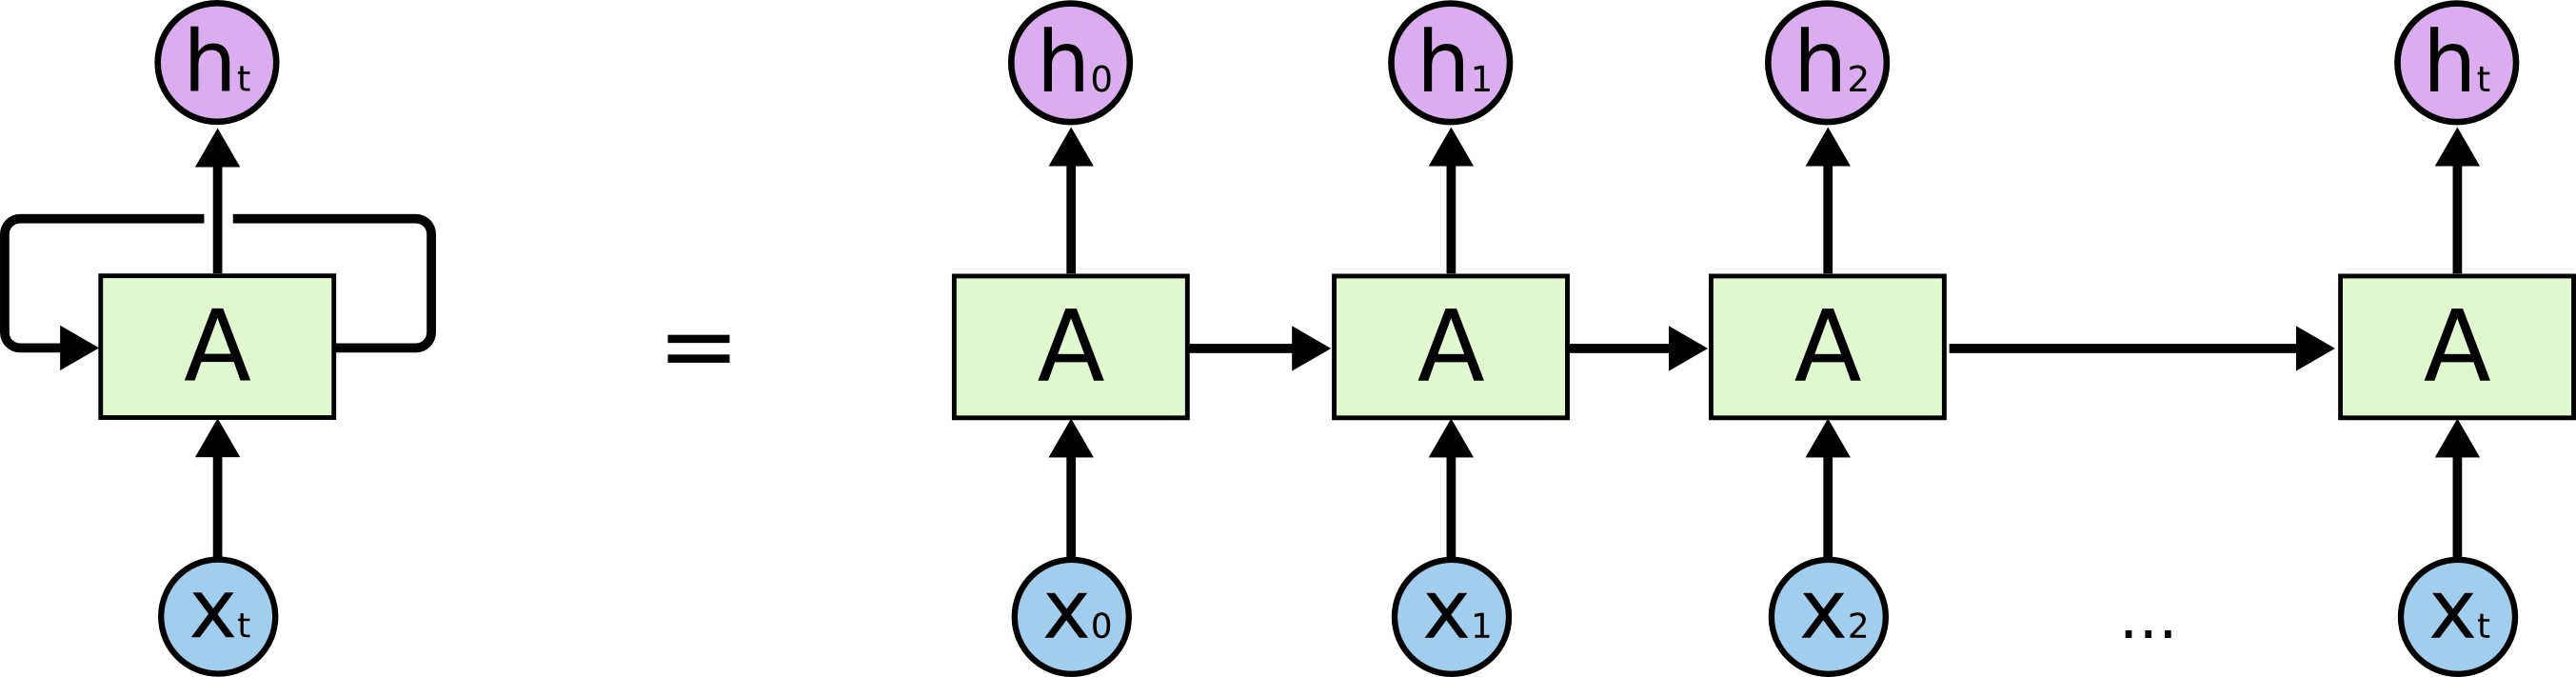
\includegraphics[width=.8\linewidth]{img/rnn}
    \caption{Rekurentinių neuroninių tinklų schema}
    \label{img:rnn}
    %http://d3kbpzbmcynnmx.cloudfront.net/wp-content/uploads/2015/09/rnn.jpg
\end{figure}
\begin{itemize}
	\item \textit{x\textsubscript{t}} - įeiga momentu \textit{t}
	\item \textit{h\textsubscript{t}} - išeiga momentu \textit{t}	
	\item \textit{A\textsubscript{t}} - būsena momentu \textit{t}	
\end{itemize}

\section{Medžiagos darbo tema dėstymo skyriai}
Medžiagos darbo tema dėstymo skyriuose pateikiamos nagrinėjamos temos detalės:
pradinė medžiaga, jos analizės ir apdorojimo metodai, sprendimų įgyvendinimas,
gautų rezultatų apibendrinimas. Šios dalies turinys labai priklauso nuo darbo
temos. Skyriai gali turėti poskyrius ir smulkesnes sudėtines dalis, kaip
punktus ir papunkčius.

Medžiaga turi būti dėstoma aiškiai, pateikiant argumentus. Tekstas dėstomas
trečiuoju asmeniu, t.y. rašoma ne „aš manau“, bet „autorius mano“, „autoriaus
nuomone“. Reikėtų vengti informacijos nesuteikiančių frazių, pvz., „...kaip jau
buvo minėta...“, „...kaip visiems žinoma...“ ir pan., vengti grožinės literatūros
ar publicistinio stiliaus, gausių metaforų ar panašių meninės išraiškos
priemonių.

\subsection{Poskyris}
Citavimo pavyzdžiai: cituojamas vienas šaltinis \cite{PvzStraipsnLt}; cituojami
keli šaltiniai \cite{PvzStraipsnEn, PvzKonfLt, PvzKonfEn, PvzKnygLt, PvzKnygEn,
PvzElPubLt, PvzElPubEn, PvzMagistrLt, PvzPhdEn}.

\subsubsection{Skirsnis}
\subsubsubsection{Straipsnis}
\subsubsection{Skirsnis}
\section{Skyrius}
\subsection{Poskyris}
\subsection{Poskyris}

\sectionnonum{Rezultatai ir išvados}
Rezultatų ir išvadų dalyje turi būti aiškiai išdėstomi pagrindiniai darbo
rezultatai (kažkas išanalizuota, kažkas sukurta, kažkas įdiegta) ir pateikiamos
išvados (daromi nagrinėtų problemų sprendimo metodų palyginimai, teikiamos
rekomendacijos, akcentuojamos naujovės).

\printbibliography[heading=bibintoc]  % Šaltinių sąraše nurodoma panaudota
% literatūra, kitokie šaltiniai. Abėcėlės tvarka išdėstomi darbe panaudotų
% (cituotų, perfrazuotų ar bent paminėtų) mokslo leidinių, kitokių publikacijų
% bibliografiniai aprašai.  Šaltinių sąrašas spausdinamas iš naujo puslapio.
% Aprašai pateikiami netransliteruoti. Šaltinių sąraše negali būti tokių
% šaltinių, kurie nebuvo paminėti tekste.

% \sectionnonum{Sąvokų apibrėžimai}
\sectionnonum{Santrumpos}
Sąvokų apibrėžimai ir santrumpų sąrašas sudaromas tada, kai darbo tekste
vartojami specialūs paaiškinimo reikalaujantys terminai ir rečiau sutinkamos
santrumpos.

\appendix  % Priedai
% Prieduose gali būti pateikiama pagalbinė, ypač darbo autoriaus savarankiškai
% parengta, medžiaga. Savarankiški priedai gali būti pateikiami ir
% kompaktiniame diske. Priedai taip pat numeruojami ir vadinami. Darbo tekstas
% su priedais susiejamas nuorodomis.

\section{Niauroninio tinklo struktūra}
\begin{figure}[H]
    \centering
    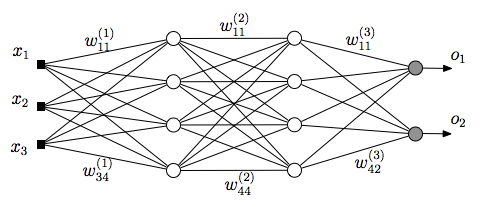
\includegraphics[scale=0.5]{img/MLP}
    \caption{Paveikslėlio pavyzdys}
    \label{img:mlp}
\end{figure}


\section{Eksperimentinio palyginimo rezultatai}
% tablesgenerator.com - converts calculators (e.g. excel) tables to LaTeX
\begin{table}[H]\footnotesize
  \centering
  \caption{Lentelės pavyzdys}
  {\begin{tabular}{|l|c|c|} \hline
    Algoritmas & $\bar{x}$ & $\sigma^{2}$ \\
    \hline
    Algoritmas A  & 1.6335    & 0.5584       \\
    Algoritmas B  & 1.7395    & 0.5647       \\
    \hline
  \end{tabular}}
  \label{tab:table example}
\end{table}

\end{document}
